\documentclass[margin=0cm]{standalone}
\usepackage{amsmath}
\usepackage{tikz}
\usepackage{pgfplots}

\pgfplotsset{compat=newest}

\usetikzlibrary{calc}
\usetikzlibrary{plotmarks}

\begin{document}
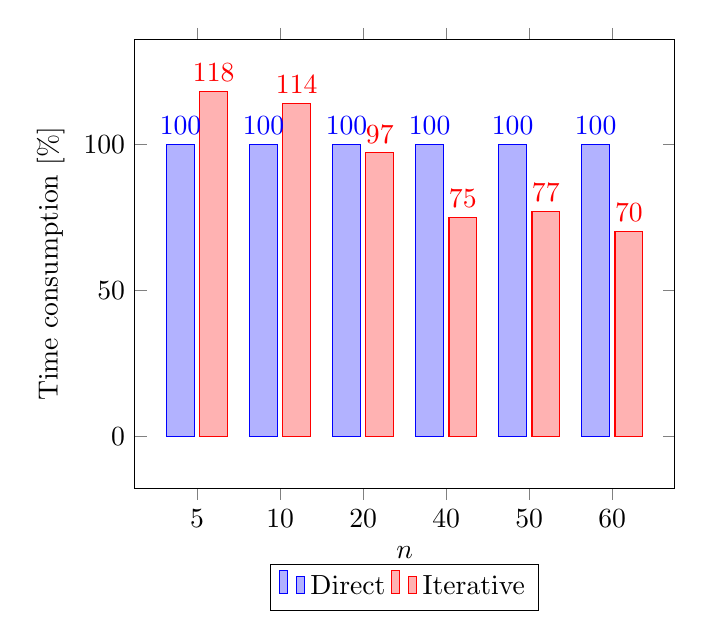
\begin{tikzpicture}
    \begin{axis}[
        ybar,
        enlargelimits=0.15,
        legend style={at={(0.5,-0.17)},
          anchor=north,legend columns=-1},
        ylabel={Time consumption [\%]},
        ymin=0,
        symbolic x coords={$5$,$10$,$20$,$40$,$50$,$60$},
        xtick=data,
        xlabel={$n$},
        nodes near coords,
        nodes near coords align={vertical},
        ]
    \addplot coordinates {($5$,100) ($10$,100) ($20$,100) ($40$,100) ($50$,100) ($60$,100)};
    \addplot coordinates {($5$,118) ($10$,114) ($20$,97) ($40$,75) ($50$,77) ($60$,70)};
    \legend{Direct,Iterative}
    \end{axis}
    \end{tikzpicture}
\end{document}
